\subsection{HTB04 - Fuse}
\subsubsection{Escaneo}
En la etapa de escaneo de puertos en la máquina, se encontró 12 puertos abiertos, teniendo de principal importante el puerto 80 con un sitio web, el puerto 135 con el servicio MSRPC y el puerto 445 con el servicio SAMBA.
\begin{figure}[H]
    \centering
    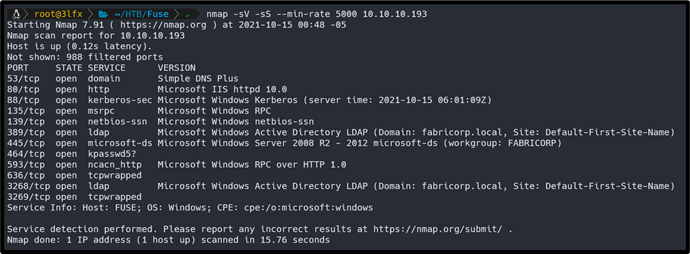
\includegraphics[width=0.99\textwidth]{imagenes/scanfuse.png}
    \caption{Escaneo de puertos Fuse}
\end{figure}
\subsubsection{Análisis de Vulnerabilidades y debilidades}
Para el análisis de vulnerabilidades, se inició revisando el sitio web levantado, al acceder nos redirigió a “fuse.fabricorp.local/papercut/logs/html/index.htm”, pero sin poder mostrarse nada, para acceder a la página se añadió el dominio en el archivo “etc/hosts” de nuestra máquina atacante. Una vez realizado, se procedió a visualizar el sitio web.
\begin{figure}[H]
    \centering
    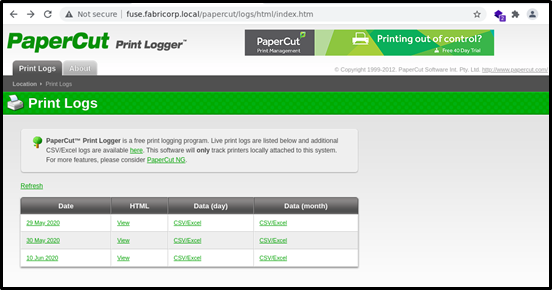
\includegraphics[width=0.99\textwidth]{imagenes/pagfuse.png}
    \caption{Página web de Fuse}
\end{figure}
Revisando la página web, se observa ciertos registros, donde se puede encontrar nombre de usuarios como se muestra a continuación (DE02).
\begin{figure}[H]
    \centering
    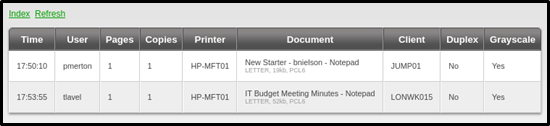
\includegraphics[width=0.99\textwidth]{imagenes/regsfuse.png}
    \caption{Página web de Fuse}
\end{figure}
A través de los registros, se consiguió adquirir 5 nombres, los cuales son: “pmerton”, “tlavel”, “sthompson”, “bhult” y “administrator”. Luego se procedió a seguir analizando el sitio web, pero no se logró más. Se buscó enumerar directorios mediante la herramienta Gobuster.
\begin{figure}[H]
    \centering
    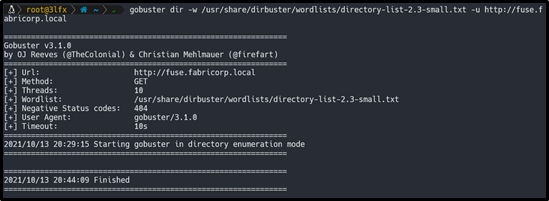
\includegraphics[width=0.99\textwidth]{imagenes/enudicfuse.png}
    \caption{Enumeración de directorios de Fuse}
\end{figure}
De esta enumeración no se logró encontrar nada, después de intentar buscar otros archivos a través de los directorios vistos anteriormente se continuo sin obtener resultado.

En este punto se procedió a revisar el servicio samba, donde se intentó acceder sin ingresar contraseña con los usuarios, pero no se tuvo éxito.
\begin{figure}[H]
    \centering
    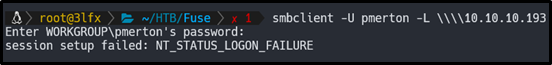
\includegraphics[width=0.99\textwidth]{imagenes/intsmbfuse.png}
    \caption{Intento de acceso al servicio samba sin uso de contraseña en Fuse}
\end{figure}
Se procedió a realizar un diccionario de contraseñas con el contenido de la página web mediante la herramienta “cewl” y se usó “hydra” para realizar fuerza bruta y encontrar una contraseña de algún usuario.
\begin{figure}[H]
    \centering
    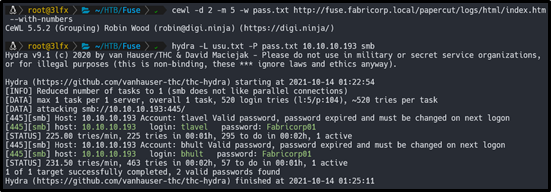
\includegraphics[width=0.99\textwidth]{imagenes/brusmbfuse.png}
    \caption{Fuerza bruta para el servicio samba en Fuse}
\end{figure}
Del proceso anterior se consiguió la contraseña de 2 usuarios, que resultaron ser la misma (DE05). Al intentar usar el comando “smbclient” con las credenciales del usuario “tlavel” nos indica que se necesita cambiar la contraseña del usuario.
\begin{figure}[H]
    \centering
    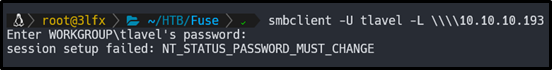
\includegraphics[width=0.99\textwidth]{imagenes/resinismbfuse.png}
    \caption{Resultado inicial al ingresar al servicio samba en Fuse}
\end{figure}
Buscando información sobre cómo realizar el cambio de contraseña, se encontró que aquella acción podía ser realizada con el comando “smbpasswd”. De forma contigua se procedió a realizar el cambio de contraseña para el usuario “tlavel”.
\begin{figure}[H]
    \centering
    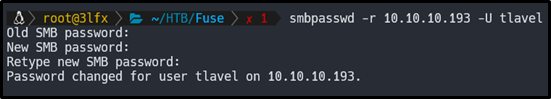
\includegraphics[width=0.99\textwidth]{imagenes/camsmbfuse.png}
    \caption{Cambio de contraseña del servicio samba en Fuse}
\end{figure}
Una vez cambiado, se accedió a los recursos permitidos por la máquina, luego se inició una búsqueda de información útil de entre los directorios, pero no se consiguió algo relevante.
\begin{figure}[H]
    \centering
    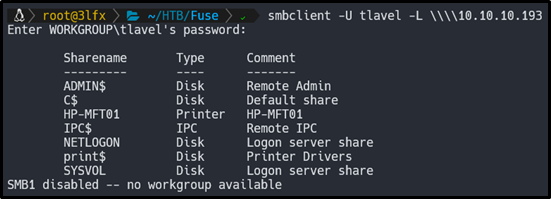
\includegraphics[width=0.99\textwidth]{imagenes/listsmbfuse.png}
    \caption{Listado de recursos compartidos por samba en Fuse}
\end{figure}
Después de no encontrar nada, se utilizó el comando “rpcclient” para conectarse y obtener más información, primero se listo los usuarios, obteniendo una mayor cantidad a la que se contaba antes.
\begin{figure}[H]
    \centering
    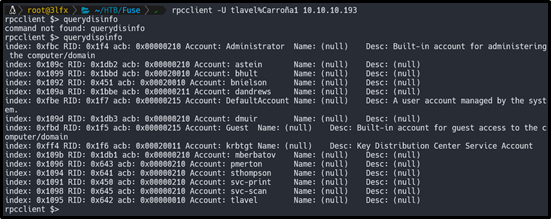
\includegraphics[width=0.99\textwidth]{imagenes/rpcclientfuse.png}
    \caption{Acceso RPCClient en Fuse}
\end{figure}
Continuando con la revisión, se llegó a buscar más información como listar privilegios, pero donde se encontró algo importante fue al enumerar impresoras, allí se encontró una contraseña (DE02).
\begin{figure}[H]
    \centering
    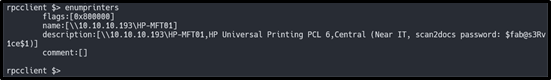
\includegraphics[width=0.99\textwidth]{imagenes/conimpfuse.png}
    \caption{Contraseña encontrada al listar imporesoras en Fuse}
\end{figure}
\subsubsection{Explotación}
Para la parte de explotación, se usó la herramienta “Evil-WinRM” perteneciente a la organización “Hackplayers” de GitHub \cite{evilwinrm}, para conectarse al sistema y se probó la contraseña encontrada con los diferentes usuarios que se había listado anteriormente, .logrando ganar acceso como el usuario “svc-print”.
\begin{figure}[H]
    \centering
    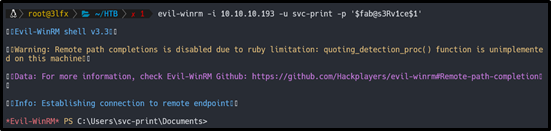
\includegraphics[width=0.99\textwidth]{imagenes/acfuse.png}
    \caption{Acceso como usuario ``svc-print'' en Fuse}
\end{figure}
\subsubsection{Escalamiento de Privilegios}
En esta fase primero se listo los privilegios que se tenía con el usuario “svc-print”. Del resultado se empezó a buscar información para escalar privilegios con estos permisos habilitados, encontrando buena información acerca del privilegio “SeLoadDriverPrivilege”.
\begin{figure}[H]
    \centering
    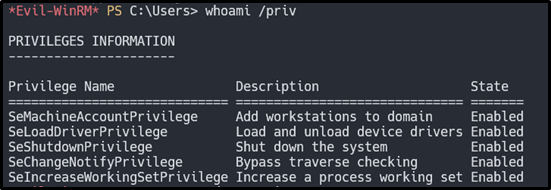
\includegraphics[width=0.99\textwidth]{imagenes/lisprivfuse.png}
    \caption{Listado de privilegios en Fuse}
\end{figure}
Para abusar del privilegio “SeLoadDriverPrivilege”, se debe cargar algún controlador que tenga alguna vulnerabilidad y permita ejecutar comandos para obtener acceso privilegiado a la máquina víctima (DE06).

Con la finalidad de realizar esto, se encontró que el controlador “Capcom.sys” era vulnerable al encontrar el explotó “ExploitCapcom” perteneciente al usuario “tandasat” de GitHub \cite{exploitcapcom}.

Revisando el código escrito en C++ del exploit, se observó que se realizaba la ejecución del CMD, pero esto generaba una terminal aparte, por ello se modificó la línea de ejecución para que se ejecute una reverse Shell que se procedería a subir, para esto se creó un directorio “C:\textbackslash{}temp\textbackslash{}” donde se subiría los archivos necesarios para nuestro escalamiento de privilegios.
\begin{figure}[H]
    \centering
    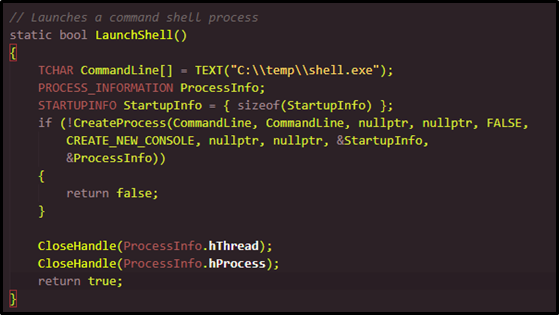
\includegraphics[width=0.8\textwidth]{imagenes/modexfuse.png}
    \caption{Modificación de exploit para Fuse}
\end{figure}
Una vez modificado el exploit se procedió a su compilación, nombrándolo como “ExploitCapcom\_csfiis.exe” al archivo ejecutable.

Luego se procedió a crear la Reverse Shell que ejecutaría el exploit modificado utilizando la herramienta “msfvenom”.
\begin{figure}[H]
    \centering
    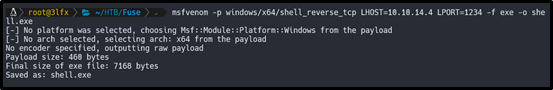
\includegraphics[width=0.99\textwidth]{imagenes/revshfuse.png}
    \caption{Creación de Reverse Shell para Fuse}
\end{figure}
Una vez generado nuestra Reverse Shell, se subió el archivo mediante nuestra sesión con “Evil-WinRM”.
\begin{figure}[H]
    \centering
    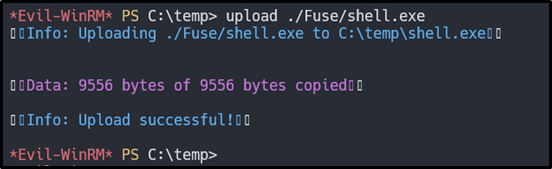
\includegraphics[width=0.8\textwidth]{imagenes/subshfuse.png}
    \caption{Subida de Reverse Shell a la máquina Fuse}
\end{figure}
También se procedió a subir el controlador “Capcom.sys” y el archivo ejecutable de la herramienta “EoPLoadDriver” perteneciente al usuario “TarlogicSecurity” de GitHub \cite{loaddriver}.
\begin{figure}[H]
    \centering
    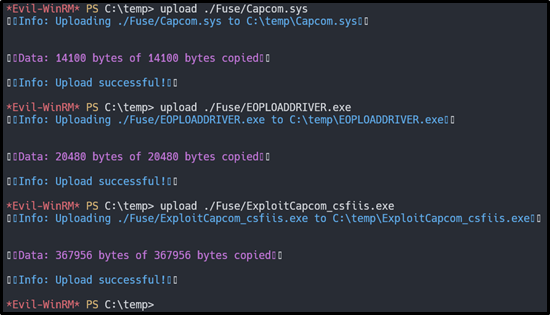
\includegraphics[width=0.99\textwidth]{imagenes/subnecfuse.png}
    \caption{Subida de archivos necesarios para escalamiento de privilegios en Fuse}
\end{figure}
Una vez subido todos los archivos necesarios, se procedió a ejecutar el programa que cargará el controlador en la máquina, cuando el programa cargó el controlador, se continúa ejecutando el exploit que modificamos.
\begin{figure}[H]
    \centering
    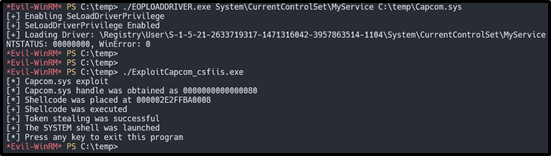
\includegraphics[width=0.99\textwidth]{imagenes/escprivfuse.png}
    \caption{Escalamiento de privilegios en Fuse}
\end{figure}
Una vez ejecutado el exploit, este realiza la ejecución de nuestra Reverse Shell con alto privilegio. Obteniendo así conexión a la máquina como “nt authority\textbackslash{}system”.
\begin{figure}[H]
    \centering
    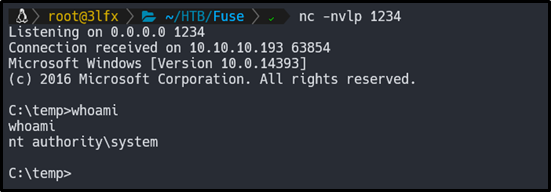
\includegraphics[width=0.8\textwidth]{imagenes/acntfuse.png}
    \caption{Acceso como ``nt authority\textbackslash{}system'' en Fuse}
\end{figure}
\subsubsection{Post-explotación}
Como parte de la post-explotación se procedio a cargar un ejecutable de la herramienta “mimikatz” a través de la sesión adquirida con el uso de Evil-WinRM.
\begin{figure}[H]
    \centering
    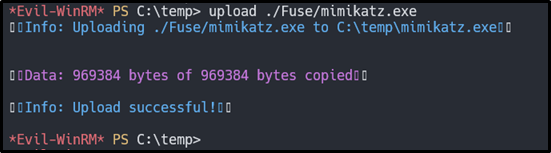
\includegraphics[width=0.8\textwidth]{imagenes/submifuse.png}
    \caption{Subida del ejecutable mimikatz a Fuse}
\end{figure}
Con este programa subido a la máquina víctima se realizó su ejecución usando privilegios elevados para su correcto funcionamiento.
\begin{figure}[H]
    \centering
    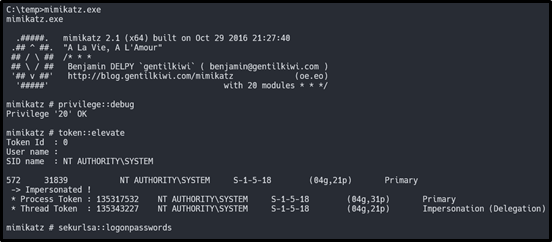
\includegraphics[width=0.99\textwidth]{imagenes/ejmifuse.png}
    \caption{Ejecución de mimikatz en Fuse}
\end{figure}
\clearpage
De manera continua se procedió a volcar los registros en el proceso LSASS para obtener contraseñas. Obteniendo una contraseña del usuario Administrador en texto plano.
\begin{figure}[H]
    \centering
    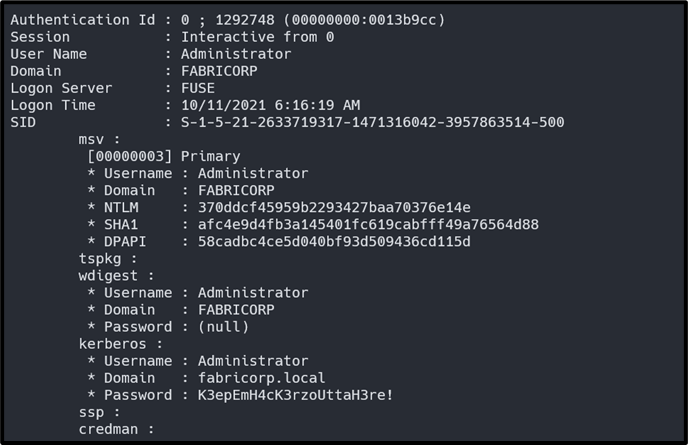
\includegraphics[width=0.9\textwidth]{imagenes/conadfuse.png}
    \caption{Contraseña en texto plano del usuario ``Administrador'' de Fuse}
\end{figure}
Con la contraseña adquirida se procedió a verificar su uso mediante la herramienta Evil-WinRM, obteniendo exitosamente una conexión a la máquina, teniendo como prueba la siguiente imagen.
\begin{figure}[H]
    \centering
    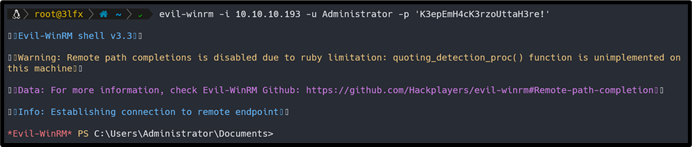
\includegraphics[width=0.99\textwidth]{imagenes/acadfuse.png}
    \caption{Acceso como usuario ``Administrador'' a la máquina Fuse}
\end{figure}
\subsubsection{Recomendaciones de mitigación}
Para evitar ataques según las debilidades encontradas en la máquina Fuse, se recomienda lo siguiente:
\begin{itemize}
    \item Realizar un control sobre la información sensible que se expone a usuarios no autorizados.
    \item Implementar requisitos más fuertes en el uso de contraseñas, con la finalidad de evitar el acceso a personas no autorizadas al contar con contraseñas fáciles de encontrar mediante fuerza bruta.
    \item Deshabilitar el permiso habilitado al usuario “svc-print” que permite la carga y descarga de controladores de dispositivo para evitar el escalamiento de privilegios.
\end{itemize}